\subsection{Two Pods Same Node}
\subsubsection{Two Pods Same Node CPU Utilization}
\begin{itemize}
    \item In the two-pods-same-node configuration, CPU utilization may be more stable compared to the single pod setup, as the workload is distributed across two pods.
    \item With two pods handling incoming requests, the load is shared, potentially reducing the CPU usage of each pod.
    \item During peak demand, CPU usage may increase as both pods manage concurrent requests on the same node.
\end{itemize}

\noindent Below is the graph that illustrates the CPU utilization for the two-pods-same-node configuration:

\begin{figure}[h]
    \begin{minipage}[t]{0.5\textwidth}
        \centering
        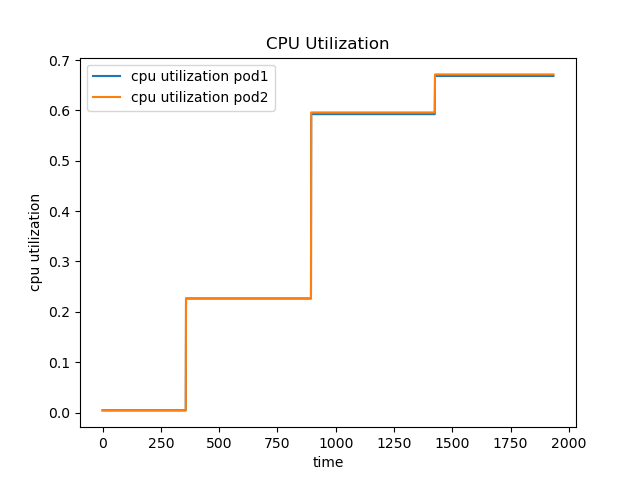
\includegraphics[width=0.9\textwidth]{../sample_results/loop/two-pod-same-node/cpu-utilization-two-pod-same-node.png}
        \caption{Loop}
    \end{minipage}
    \hfill
    \begin{minipage}[t]{0.5\textwidth}
        \centering
        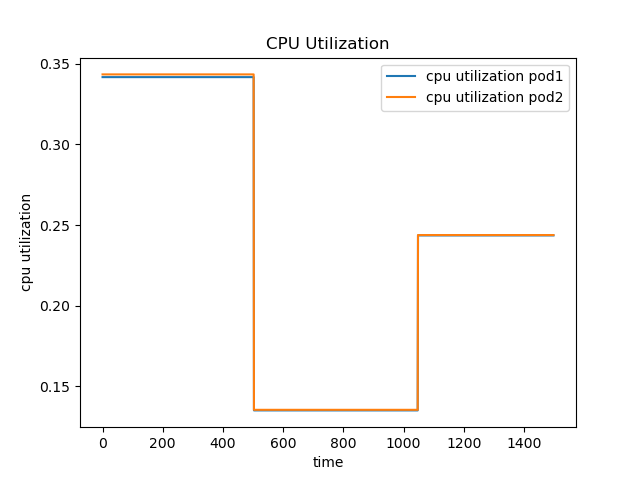
\includegraphics[width=0.9\textwidth]{../sample_results/lorem/two-pod-same-node/cpu-utilization-two-pod-same-node.png}
        \caption{Lorem}
    \end{minipage}
\end{figure}

\newpage
\subsubsection{Two Pods Same Node Response Time Observations}
\begin{itemize}
    \item Response times in the two-pods-same-node configuration can be consistent, as two pods share the workload.
    \item If one pod is under heavy load, the other can manage additional requests, balancing response times.
    \item This setup helps maintain consistent response times as the workload is distributed across both pods.
\end{itemize}

\noindent Below are the response time graphs for the two-pods-same-node configuration:

\begin{figure}[h]
    \begin{minipage}[t]{0.5\textwidth}
        \centering
        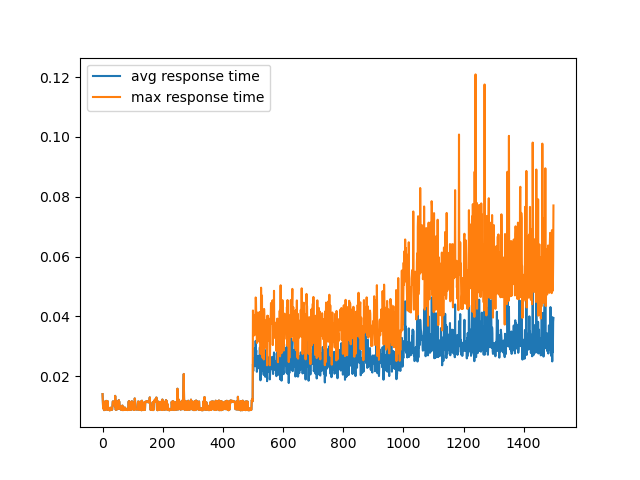
\includegraphics[width=0.9\textwidth]{../sample_results/loop/two-pod-same-node/response-time-two-pod-same-node-two-pod-same-node.png}
        \caption{Loop}
    \end{minipage}
    \hfill
    \begin{minipage}[t]{0.5\textwidth}
        \centering
        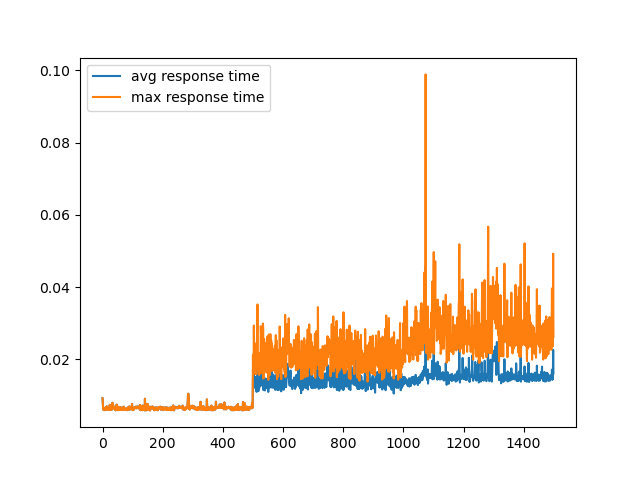
\includegraphics[width=0.9\textwidth]{../sample_results/lorem/two-pod-same-node/response-time-two-pod-same-node-two-pod-same-node.png}
        \caption{Lorem}
    \end{minipage}
\end{figure}

\newpage
\subsubsection{Two Pods Same Node Memory Utilization}
\begin{figure}[h]
    \begin{minipage}[t]{0.5\textwidth}
        \centering
        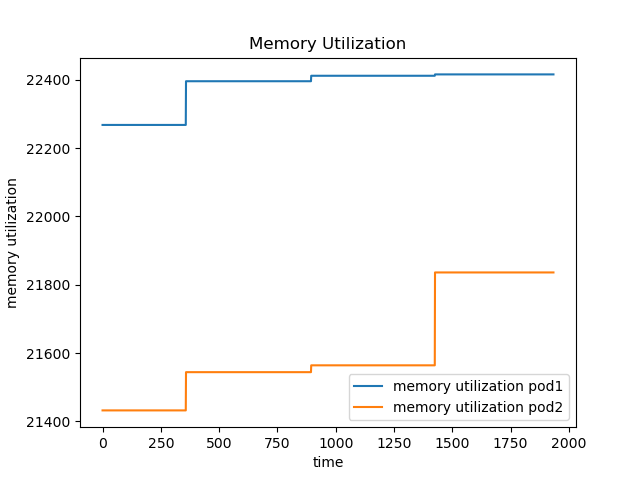
\includegraphics[width=0.9\textwidth]{../sample_results/loop/two-pod-same-node/mem-utilization-two-pod-same-node.png}
        \caption{Loop}
    \end{minipage}
    \hfill
    \begin{minipage}[t]{0.5\textwidth}
        \centering
        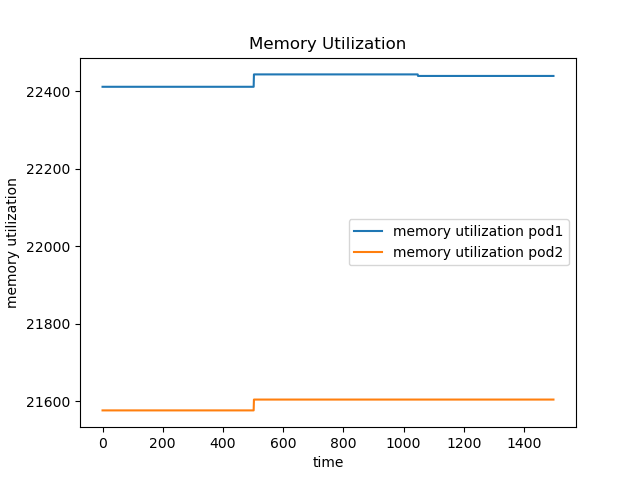
\includegraphics[width=0.9\textwidth]{../sample_results/lorem/two-pod-same-node/mem-utilization-two-pod-same-node.png}
        \caption{Lorem}
    \end{minipage}
\end{figure}

\begin{itemize}
    \item Memory utilization in the two-pods-same-node configuration can vary based on the workloads and the memory requirements of each pod.
    \item Since two pods share the same node, memory usage might be affected by how each pod manages its resources.
    \item As workloads stabilize, memory utilization tends to balance out as both pods handle their own resource management.
\end{itemize}

